\chapter{序論}
本研究にて,ユーザが定義した手書きジェスチャを高速に認識し,かつどのような開発環境においても実装可能な軽量なアルゴリズムを示す.
本章にて,まず初めに研究背景として既存の手書きジェスチャ認識手法とその課題を述べる.次にその課題を解決すべく本研究の目的を述べ,最後に本論文の構成を述べる.

\section{背景}
スマートフォンやタブレット端末のタッチパネルへの入力手法として,ペンや指を用いた手書きジェスチャが多く採用されている.特にそれらを入力として用いるようなアプリケーションをプロトタイピングする環境において,手書きジェスチャをアプリケーションに組み込む際に求められることとして,~\cite{Rettig:1994:PTF:175276.175288}において述べられているように,手書きジェスチャ認識を実現するためのパターン認識に関する専門的な知識~\cite{Hong00constructingfinite, Anderson2004HiddenMM,Sezgin:2005:HES:1040830.1040899, Cao:2005:EOA:1089508.1089540, Pittman:1991:RHT:108844.108914, Cho:2006:NGR:1711617.1711649,Rubine:1991:SGE:127719.122753, Anthony:2010:LMR:1839214.1839258}がなくとも,素早く実装できること(すなわち複雑な数式やアルゴリズムを用いていないということ),素早く手書きジェスチャ入力のテストができること(すなわちあまり学習データを必要としないこと)などが挙げられる.同時に,ジェスチャ認識であるため,認識率が高いこと,認識速度が速いことも求められる.また,手書きジェスチャは,入力されるジェスチャの形状が毎回微妙に異なる可能性が高いため,たとえ形状が微妙に異なったとしても意図したジェスチャとして正しく認識されるようなロバスト性の高い認識アルゴリズムであることも求められる.また,学習データをあまり必要としないということは,アプリケーションユーザが独自に手書きジェスチャを定義することが可能なシステムを実現することにもつながり,これも手書きジェスチャを入力として用いるアプリケーションを開発する多くの開発者によって求められていることの1つである.

\$1~\cite{Wobbrock:2007:GWL:1294211.1294238}は,まさにこれらの要件を満たす手書きジェスチャ認識アルゴリズムであり,「アルゴリズムが簡潔である,少ない学習データにおいて高い認識率を示す,認識速度が速い,ロバスト性が高い」といった特徴を持ち,単一ストロークからなる手書きジェスチャを認識可能なアルゴリズムである.\$1は,現に,ActionScript, Python, C\#, C++, Objective-C, Java, Java ME, and JavaScriptといった言語において実装されている.
そのため,多くの開発者にとって,手書きジェスチャ認識を自身のシステムに組み込むことが容易となった.特に手書きジェスチャ認識のためのライブラリが存在しないようなプロトタイピング開発環境において,その存在価値は非常に高い.また,\$1を改良した多くのアルゴリズムは\$-Family Recognizer~\cite{Anthony:2010:LMR:1839214.1839258,Reaver:2011:MQU:2021164.2021183,Li:2010:PFA:1753326.1753654,Anthony:2012:NFA:2305276.2305296,Herold:2012:CRF:2331067.2331074,Vatavu:2012:GPC:2388676.2388732,Taranta:2015:PPB:2788890.2788925,Pittman:2016:FFA:2856767.2856808,Vatavu:2012:OAF:2166966.2167022,}として知られ,\$1の持つ「アルゴリズムが簡潔である」という特徴を維持しつつ,認識率や認識速度の向上,識別可能なジェスチャの種類の増加といった観点から改良が試みられた.ペンや指を入力として用いるようなインタフェースが普及し,それらを用いたアプリケーションの開発者が増加している今日において,これらアルゴリズムは,手書きジェスチャ認識を自身のシステムに容易に組み込むための手段として必要とされており,アルゴリズムの開発・改良の機運が高まっている.
これまで開発されてきた\$-Family Recognizerは,ジェスチャを構成するストロークの,大きさ,向き,位置に関して,そのいずれかあるいはすべてについて不変になるようなアルゴリズムを採用することにより,不変にしたものについてロバストなジェスチャ認識を実現した.これらアルゴリズムにおいては,手書きジェスチャの書き順が同じでありかつ手書きジェスチャを構成するストロークの形状さえ類似していれば,ストロークの大きさ,向きあるいはストロークが入力された位置などが多少異なっても,同じ形状と書き順の手書きジェスチャとして認識される.その結果,認識率の向上が実現された.
それらを不変にしない,つまり特徴量として認識のために用いるということは,その特徴量について識別できるため,識別可能な手書きジェスチャが増加することにつながるが,不変にしない特徴量についてはロバストではなくなるため,認識率の低下を招く恐れがある.
例えば,Rubine Classfier~\cite{Rubine:1991:SGE:122718.122753}は13もの手書きジェスチャの特徴量を用いることにより手書きジェスチャを認識し,手書きジェスチャを構成するストロークの形状と書き順は同じであるが,大きさ,向き,位置に関して異なるジェスチャ~(図\ref{fig:examples_V})を識別することが可能である.しかしながら,認識に用いる特徴量が多いため,結果的に認識率の低下を招いている.

\begin{figure} [htbp]
\centering
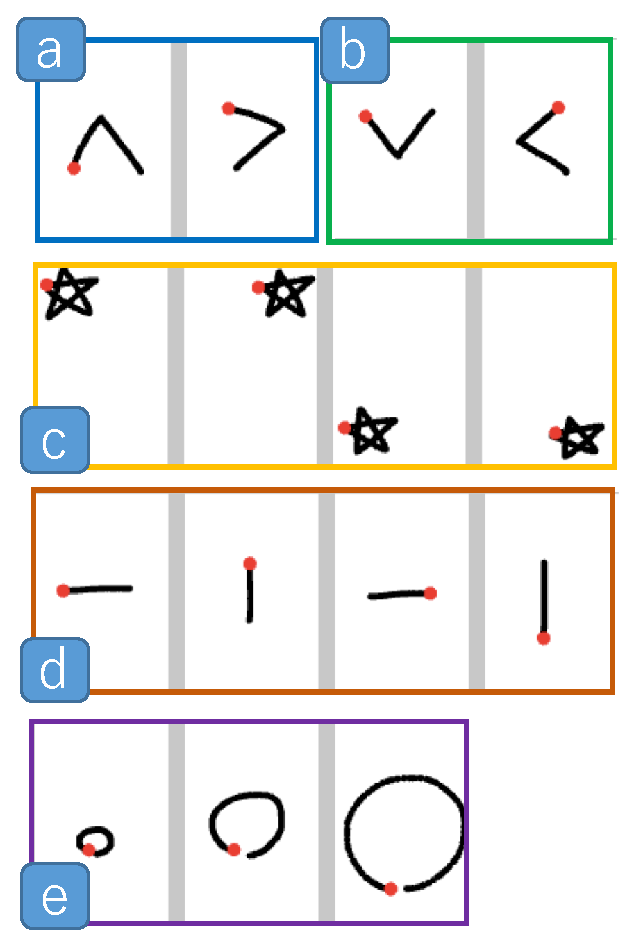
\includegraphics [width=0.5\columnwidth]{img/examples_V.eps}
\caption{ストロークの形状と書き順は同じであるが,大きさ (e), 向き (a) (b) (d), 位置 (c) が異なる,単一ストロークからなる手書きジェスチャの例}
\label{fig:examples_V}
\end{figure}


認識速度の観点でいえば,DTW~\cite{Tappert:1982:CSR:1664966.1664979, Salvador:2007:TAD:1367985.1367993}は,HCI分野において,手書きジェスチャ認識を実現するために広く採用されているアルゴリズムであり,単純にストロークを構成する点の距離を比較するのみであるため,こちらも,手書きジェスチャを構成するストロークの形状と書き順は同じであるが,大きさ,向き,位置に関して異なるストロークを識別することは可能である.しかしながら,単純なアルゴリズムによって認識率を向上させるために,非常に計算量が大きいといった問題点がある.

しかしながら,ユーザ調査により,これまでに述べたきたような,ストロークの形状と書き順は同じであるが,大きさや向きや位置が異なる単一ストロークからなる手書きジェスチャ~(図\ref{fig:examples_V})をアプリケーションユーザが入力として用いることを要望していることが導かれた.
これらは既に述べたように既存の\$-Family Recognizerにおいて識別できないため,これらのようなユーザ定義手書きジェスチャを入力として用いるようなアプリケーションを開発したい開発者は既存の\$-Family Recognizerを認識アルゴリズムとして用いることができない.また,これらを識別可能なRubine classfierやDTWなどを採用した場合は,認識率や認識速度において十分なパフォーマンスを得られない可能性がある.


\section{目的}
本研究の目的は,\$1を拡張し,単一ストロークからなる手書きジェスチャに対し,ストロークの大きさ,向き,位置に関して識別可能としながらも,\$1と比較し認識率の低下と認識速度の低下を最小限に抑えることを実現した\$-Family Recognizer開発することである.
我々はこの,ストロークの大きさ,向き,位置に関して``V''ariant~(不変)なストロークを認識する\$-Family Recognizerを\$Vと名付けた.
\$Vは\$1にアルゴリズムを少し追加するのみであるため,どのような開発環境においても実装可能であることも目標としている.
また,\$1と同様,少ない学習データにおいて高い認識率を示すことも目標としており,これは,アプリケーションユーザが手書きジェスチャを独自に定義することが可能であることを示している.
また,大きさ,向き,位置に関して識別可能な既存アルゴリズムと比較することによって,\$Vの有用性を示すことも本研究における目的とする.


%\$Vは,大きさ,向き,位置を特徴量として用いることによって,それらに依存するストロークを識別可能とした.
%その際,学習データを元に,ストロークを形状と書き順ごとに分類し,認識に用いる特徴量に重み付けをすることによって考慮すべき特徴量を適切に配分し,\$1と比べても遜色のない認識率と認識速度を実現した.
%\$1を改良した多くのアルゴリズムを用いず,\$1を拡張した理由は,\$1にて計算された,大きさ,向き,位置の特徴量を再利用することによって,\$1アルゴリズムと比べて,アルゴリズムの追加量を抑えること,認識速度の低下を抑えることにつながるからである.

\section{貢献}
本研究における手書きジェスチャ認識アルゴリズム\$Vの貢献を以下に示す.
\begin{itemize}
\item 手書きジェスチャを構成するストロークの形状と書き順は同じであるが,大きさ,向き,位置に関して異なる手書きジェスチャ識別することが可能なアルゴリズムを開発した.
\item 少ない学習データにおいて認識率を向上させるためのアルゴリズムを開発した.
\item 認識速度を向上させるためのアルゴリズムを開発した.
\item どのような開発環境においても実装可能な軽量なアルゴリズムを開発した.
\end{itemize}

\section{本論文の構成}
第1章では,研究背景と目的を述べた.第2章では,関連研究を述べる.第3章では,本研究の動機にもなった,アプリケーションユーザが入力として用いたい手書きジェスチャの調査について述べる.第 4 章では,\$Vの拡張元である\$1アルゴリズムについて述べ,第5章において,\$Vアルゴリズムの詳細について述べる.第6章では,\$Vのアルゴリズムとしての性能評価実験について述べる.第7章では,\$Vを用いたアプリケーション例を述べる.第8章では,\$Vアルゴリズムの今後の展望について議論する.第9章では,本研究の結論を述べる.
なお,付録 A に\$Vアルゴリズムの擬似コードを示す.
%付録 B に第 3章のユーザ調査に用いた調査同意書を,付録 B に調査について説明する際に用いた説明書を,付録 Dに第6章の評価実験に用いた実験同意書を示す.
